\section{Three-Hump Camel Function}
\label{sec:app:test:three-hump}
  The \emph{Three-Hump Camel function}, colloquially termed as the camel-back 
  function, serves as a standard benchmark in the optimization algorithms
  testing landscape.
  This two-dimensional function earns its name from the characteristic tri-modal
  hump visual pattern it presents in a three-dimensional space, bearing
  resemblance to a camel's back.

  \begin{definition}[Three-Hump Camel Function]
    \label{def:app:test:three-hump}
    The \emph{Three-Hump Camel function}, depicted as \(f: \mathbb{R}^2 \rightarrow 
    \mathbb{R}\), is formally expressed as:

    \begin{equation}
      \label{eq:app:test:three-hump}
      f(x,\,y) = 2x^2 - 1.05x^4 + \frac{x^6}{6} + xy + y^2
    \end{equation}
    
    where \(-5 \leq x \leq 5\) and \(-5 \leq y \leq 5\).
  \end{definition}

  The Three-Hump Camel function exhibits its global minimum at the origin,
  \(f(0,\, 0) = 0\).
  Although its form appears straightforward, the function's multiple local
  optima pose considerable challenges for optimization algorithms, making it an
  excellent test case.

  \begin{figure}[ht!]
    \centering
    \begin{subfigure}[b]{0.45\textwidth}
      \centering
      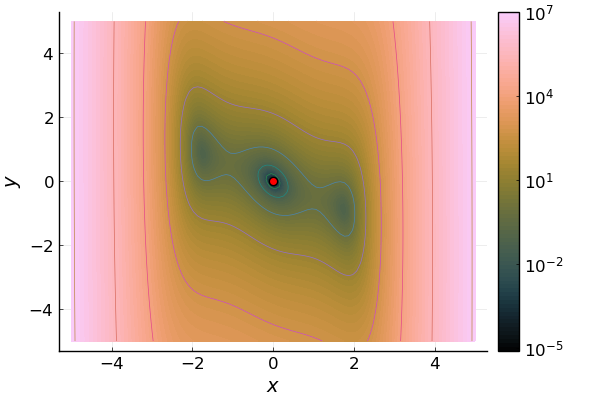
\includegraphics[width=\textwidth]{img/test_functions/three_hump_camel_contour.png}
      \caption{
        Contour plot of the Three-Hump Camel function.
        The red dot signifies the global minimum.
      }
      \label{fig:app:test:three-hump:contour}
    \end{subfigure}
    \hfill
    \begin{subfigure}[b]{0.45\textwidth}
      \centering
      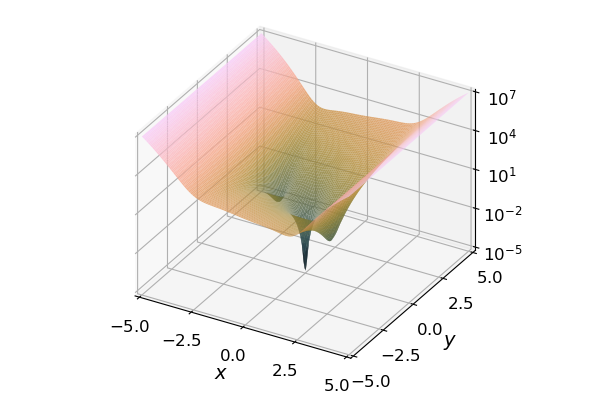
\includegraphics[width=\textwidth]{img/test_functions/three_hump_camel_surface.png}
      \caption{
        Surface plot showcasing the characteristic tri-modal humps of the
        Three-Hump Camel function.
      }
      \label{fig:app:test:three-hump:surface}
    \end{subfigure}
    \caption{Contour and surface visualizations of the Three-Hump Camel function}
    \label{fig:app:test:three-hump}
  \end{figure}
